% last updated in April 2002 by Antje Endemann
% Based on CVPR 07 and LNCS, with modifications by DAF, AZ and elle, 2008 and AA, 2010, and CC, 2011; TT, 2014; AAS, 2016

\documentclass[runningheads]{llncs}
\usepackage{graphicx}
\usepackage{amsmath,amssymb} % define this before the line numbering.
\usepackage{ruler}
\usepackage{color}
\usepackage[width=122mm,left=12mm,paperwidth=146mm,height=193mm,top=12mm,paperheight=217mm]{geometry}
\begin{document}
% \renewcommand\thelinenumber{\color[rgb]{0.2,0.5,0.8}\normalfont\sffamily\scriptsize\arabic{linenumber}\color[rgb]{0,0,0}}
% \renewcommand\makeLineNumber {\hss\thelinenumber\ \hspace{6mm} \rlap{\hskip\textwidth\ \hspace{6.5mm}\thelinenumber}}
% \linenumbers
\pagestyle{headings}
\mainmatter
\def\ECCV18SubNumber{31}

\title{Self-Driving Assistant in Computer Simulation 
Environment}

\titlerunning{ENGN4528 Group \ECCV18SubNumber}

\authorrunning{ENGN4528 Group \ECCV18SubNumber}

\author{Zhiyuan Chen, Xingyuan Xu, Qiusi Xiang, Bisyri 
Hisham, Kavinenh Mohanraj}
\institute{Australian National University}


\maketitle

% FORMAT GUIDE
% No more than 60 characters in a single line [1][2]
% All lines must ends with a whitespace
% Every section ends with two empty lines
% Every subsection ends with a empty line
% [1]: Punctuation at the end of the line does not count
% [2]: Whitespace at the end of the line does not count

\begin{abstract}
This project implements a self-driving assistant in 
computer simulation environment with Spatial CNN for lane 
line detection and Mask R-CNN for objects detection on a 
distributed system based on RabbitMQ, Docker, and 
Kubernetes.
\dots
\keywords Self-Driving, Spatial CNN, Mask R-CNN, 
Distributed System
\end{abstract}


\section{Introduction}
Self-driving technologies had been used in airplanes (known 
as AP for Auto Pilot), and trains (known as ATO for 
Automatic Train Operation) for decades. However, as 
road traffic is far more complex, self-driving cars have 
never been in commercial use. Thanks to the development of 
Machine Learning, Computer Vision and most importantly the 
hardwares, self-driving cars does not seem to be impossible 
nowadays. Thus, we have designed a self-driving assistant program 
which detects the lane line and objects in a computer 
simulation environment. 


\section{Manager Process}
\subsection{Screenshot}
Taking a screenshot can be harder than it looks. 
ImageGrab.grab() from PIL is a good approach. However, 
it costs 300-400ms to take a single screenshot which is 
obviously unacceptable. We have tested many different functions 
from different packages, and as a result, Python-MSS is much 
faster than any other packages in comparison with an 
average speed of 60fps, and was used at last.

\subsection{Encode \& Decode}
As we are using message queue as our message-oriented 
middleware, we must encode(serialize) the image prior to 
transmission and decode(deserialize) upon receiving messages. 
We tried three different ways to encode our image, JSON, 
pickle, and imencode. 

JSON is widely used in message queue, however, as ndarray 
used for image cannot be directly converted to JSON, we have 
to serialize the image first. Multiple attempts have been 
made, we succeeded in encoding the image in milliseconds at last, 
unfortunately, we could not decode the image fast enough 
and we had to abandon JSON. 

Directly pack the image using pickle can be another method, 
we tried cPickle here instead for better performance. The 
encode and decode speed is the best among all other methods, 
however, the size of the message is also several times 
larger than the size of the image. Messages of this size 
would place a heavy burden on the network, and was finally 
deprecated. 

The Joint Photographic Experts Group issued a synonym 
standard for still pictures compression in 1992, after 
27 years, the JPEG algorithm had became the most commonly 
used algorithm in image compression on this planet. OpenCV 
provides a built-in function, i.e. imencode, which can 
convert a image from ndarray to byte stream within 
milliseconds. And more importantly, thanks to JPEG 
algorithm, the size of message is also ideal. 

Therefore, we are managed to reduce the transmission 
latency, i.e. encode image, transmit to worker, decode 
image, encode image, transmit to manager, within 0.05 seconds.

\begin{figure}
    \centering
    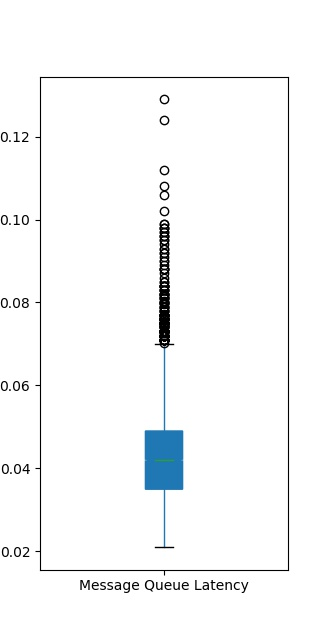
\includegraphics[height=6cm]{reference/latency}
    \label{fig:MQLatency}
    \caption{Message Queue Latency}
\end{figure}


\section{Worker Process}

\subsection{Lane Line Detection}
Lane line detection has always been one of the most 
important part of self-driving. This is easy to understand 
since driving off road usually means car crash and severe 
injuries. 

Traditionally, we first use affine transformation to obtain 
the aerial view of the lane line. Then, we use edge 
detector, e.g. Canny, Sobel, as well as gradient to enhance 
the image. After the image process, we use sliding windows 
to locate the lane line. Lastly, we project the lane line 
back to the original image, and calculate the radius and 
distance to center. 

However, the traditional strategy does not have steady 
outputs, it would be easily influenced by curved roads, 
shadows, and others. It can neither process rural roads or 
trails without actual lines on the ground. Thus, most 
modern lane line detector use convolutional neural network 
(CNN) instead, we are no exception. 

We compared two different CNN, i.e., LaneNet, and 
Spatial CNN in this project to achieve the best performance. 

LaneNet was suggested by Wang et al.\cite{LaneNet} in 2018. 
They proposed to cast the lane detection problem as an 
instance segmentation problem so that it can be trained 
end-to-end which could better cope with lane changes. 
They split the image to background and lanes instead of 
assign different classes to different lanes. By doing so, 
they are able to solve the problems of lane switching and 
limitation of the number of lanes. They started by binary 
segment the lane line with background first. They connect 
all ground-truth lane points together to form a connected 
line per lane so that it works well even though the lane 
line are occluded by objects like vehicles. Then, they 
instance segment the lane line with each other using a 
one-shot method based on distance metric learning. It use a 
clustering loss function to cluster points into lanes using 
the distance between pixel embeddings.
 
\begin{figure}
    \centering
    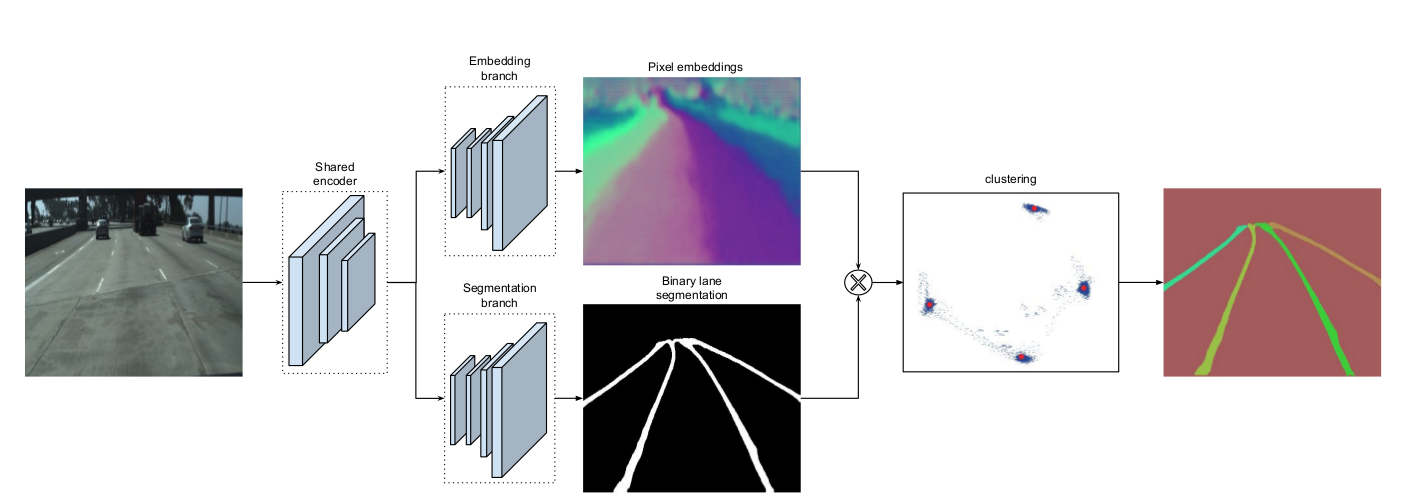
\includegraphics[width=8cm]{reference/lanenet}
    \label{fig:LaneNet}
    \caption{Network architecture of LaneNet}
\end{figure}

Spatial CNN (SCNN) was proposed by Pan et al.
\cite{SpatialCNN} in 2017. They generalize traditional 
deep layer-by-layer convolutions to slice-by-slice 
convolutions within feature maps, which can enable message 
passings between pixels across rows and columns in a layer. 
It allows space information to propagate in the same layer 
and make SCNN much more suitable to recognize structure 
objects. As a result, Spatial CNN won the TuSimple Lane 
Detection Challenge with 96.53\%. 

\begin{figure}
    \centering
    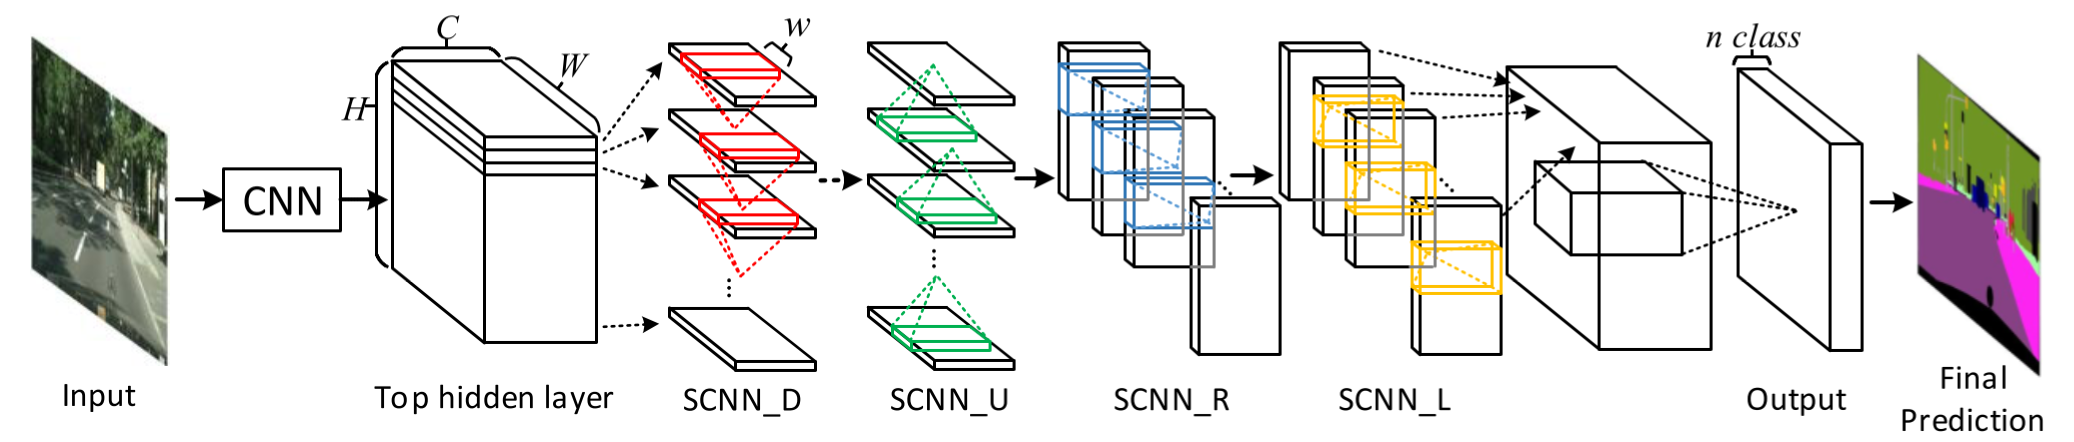
\includegraphics[width=8cm]{reference/scnn}
    \label{fig:SCNN}
    \caption{Network architecture of Spatial CNN}
\end{figure}

\begin{table}[!htbp]
	\centering
	\begin{tabular}{|l|c|c|}
		\hline 
		&LaneNet&Spatial CNN\\
		\hline  
		Accuracy (\%)&96.4&96.53\\
		\hline  
		Speed (fps)&52&90\\
		\hline 
	\end{tabular}
	\caption{Test run on TuSimple dataset}
\end{table}

After comparison, we found that SCNN works better than 
LaneNet in both speed and accuracy. Thus, we chose to use 
the SCNN in our project. 


\subsection{Obstacle Detection}
Prior to the introduction of Region-based Convolutional 
Neural Networks (R-CNN) suggested by Girshick et al. 
\cite{RCNN} in 2013, visual recognition tasks has been 
based considerably on the use of Histograms of Oriented 
Gradients (HOG)\cite{HOG}, and Scale-Invariant Feature 
Transform (SIFT)\cite{SIFT}. However, as the recognition of 
brain occurs in several stages downstream, we could assume 
that a hierarchical, multi-stage algorithm can do better in 
recognition task. 

Girshick et al. work on R-CNN showed us a new approach in 
pattern recognition. Compare to classification of image, 
recognition needs to localizing the objects first. 
Traditionally, it is considered as a regression problem. 
They used selective search to extract around 2000 region 
proposals. Then, they used a CNN to extract a 
4096-dimensional feature vector from each region proposal. 
After that, they computed features by forward propagating
a mean-subtracted 227 × 227 RGB image through five 
convolutional layers, and two fully connected layers. At 
last, they used a Support Vector Machine to classify the 
feature vectors, and a Bounding-box regression to get the 
ground truth box. 

\begin{figure}
    \centering
    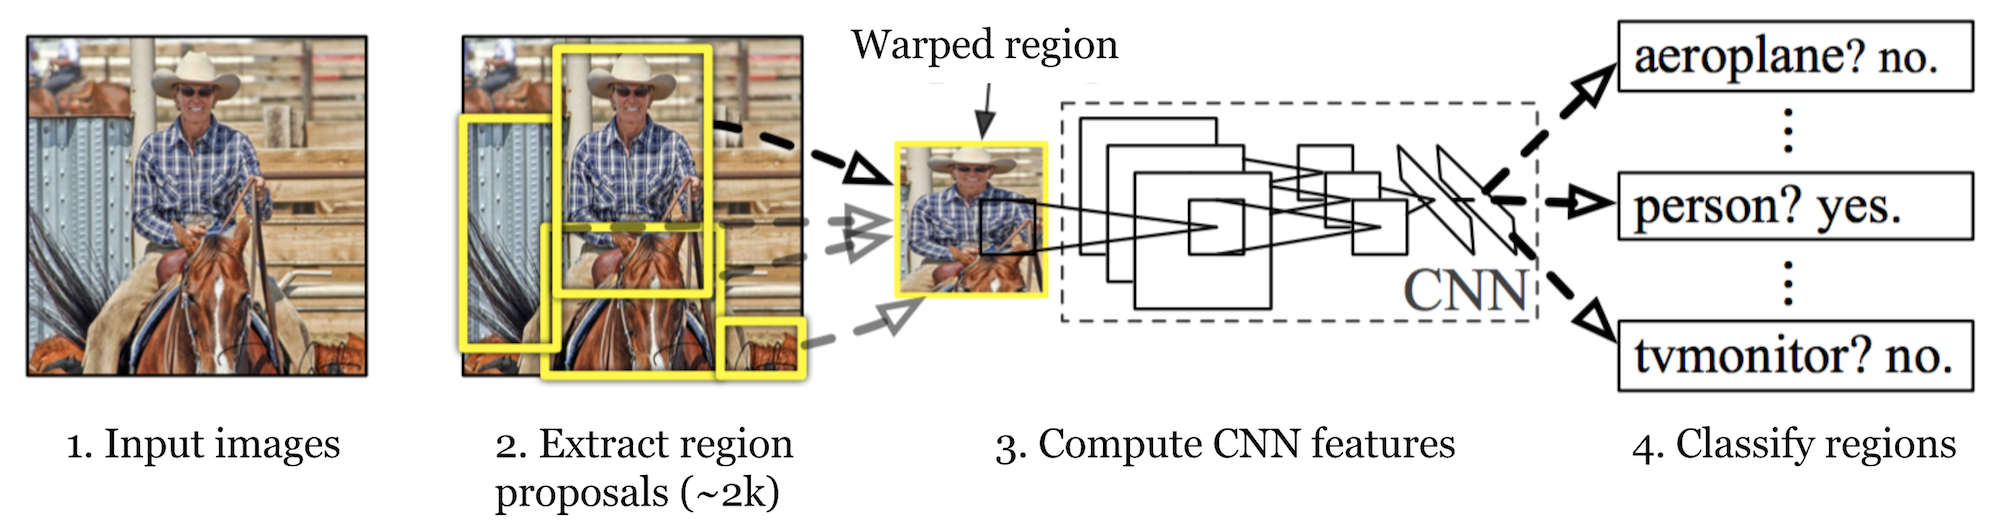
\includegraphics[width=8cm]{reference/rcnn}
    \label{fig:RCNN}
    \caption{Network architecture of R-CNN}
\end{figure}

We compared two different variants of R-CNN, i.e., 
Faster R-CNN, and Mask R-CNN in this project to achieve the 
best performance. 

Faster R-CNN\cite{FasterRCNN} (FRCNN) was suggested by Ren 
et al. in 2015. Similar to R-CNN, FRCNN used CNN to 
extract features from region proposals, however, unlike 
R-CNN, FRCNN used a Region Proposal Network (RPN) instead 
of selective search to localize the region proposals. In 
addition, a ROI pooling layer was added between RPN and 
CNN, it is used to collect proposals, and calculate the 
proposal feature maps to extract features. Besides, FRCNN 
use fully-connected layer, and softmax to classify the 
features like Fast R-CNN instead of SVM. 

\begin{figure}
    \centering
    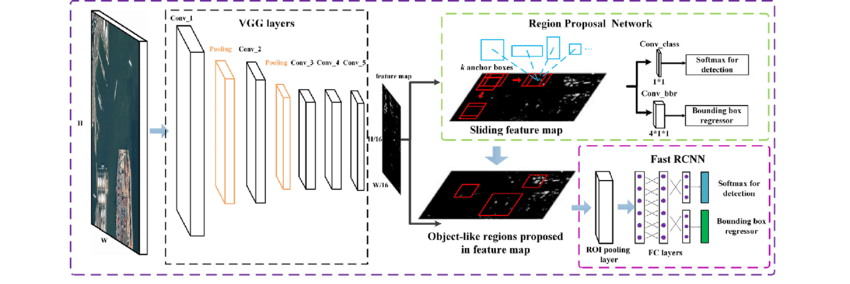
\includegraphics[width=8cm]{reference/frcnn}
    \label{fig:FRCNN}
    \caption{Network architecture of FRCNN}
\end{figure}

Mask R-CNN\cite{MaskRCNN} (MRCNN) was proposed by He et al. 
in 2018. As the feature image and original image in Faster 
R-CNN is mis-alignment due to ROI polling, MRCNN changes ROI 
polling with ROIAlign. In addition, MRCNN adds a 
convolutional layer after ROIAlign to predicate the mask. 

\begin{figure}
    \centering
    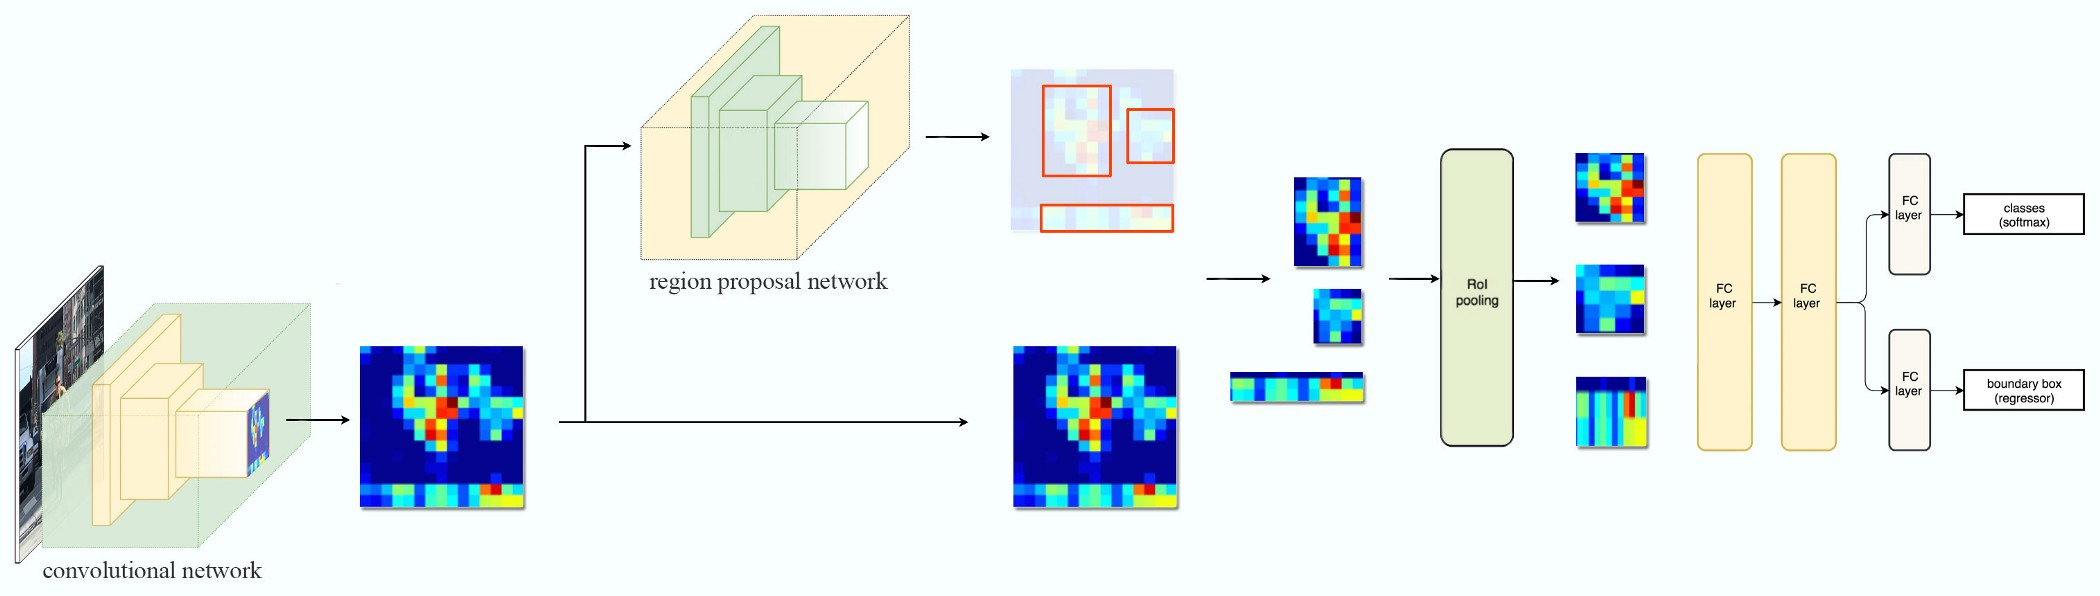
\includegraphics[width=8cm]{reference/mrcnn}
    \label{fig:MRCNN}
    \caption{Network architecture of mrcnn}
\end{figure}

Since the MRCNN outputs the result of segmentation and 
detection in parallel, the result can be better. Thus, 
we chose to use MRCNN in this project to detect objects.


\section{Distributed System}

\subsection{Message-Oriented Middleware}
Message-Oriented Middleware or MOM was used to transmit 
data between each cluster, and is the core of the whole 
distributed system. MOM deliver messages asynchronously 
which benefits us a lot. It allows us to remove 
dependencies between each algorithm and decouple our 
program. Moreover, it also increases the reliability of our 
program, since the system would continue to work even 
though one or more of the algorithms encountered fatal 
problems, and unable to recover.

Message Queue was used in our program as the MOM. We 
compared many message queues, including kafka, RabbitMQ, 
NATS, and Redis to find the best performed message queue 
in latency. As Advanced Message Queueing Protocol 
implementation, kafka and RabbitMQ are a lot slower than 
Redis and NATS in 1KB and 5KB text. However, when it comes
to 1MB text, RabbitMQ and kafka are 200 times faster than 
NATS and Redis in 99.99th percentile. Thus, we chose 
RabbitMQ as our MOM since it works slightly better in large 
message transmission. In addition, to improve the real-time 
capabilities, a Time To Live limit is set to 1 millisecond.


\subsection{Containerization}
Containerization has been widely used in many industries. 
Compare to traditional virtual machine, the performance, 
and resources loss are reduced to a large extent benefits 
from removing the guest OS, and hardware virtualization. 
Moreover, using container would also reduce the effort to 
deploy in future works. 

Docker, the most popular container platform, are used here 
in this project to containerize our algorithm. Compare to 
other containerization strategy, e.g. LXD, Docker focused 
on running programs instead of a whole system which makes 
it easier to use. In addition, Docker also supports multiple 
system which is more convenient for development. And most 
importantly the nvidia-docker makes Docker more compatible 
with neural networks.

\subsection{Container Orchestration}
As our application runs on multiple containers, a container 
orchestration platform which can help us manage and scale 
our containers is also necessary. Docker Swarm was implemented 
first as it is built in the Docker CE but soon deprecated 
since Docker Swarm does not provide basic heal-checks 
and auto-rollback. Rancher provides more useful functions, 
however, since it does not have good support on 
nvidia-docker, we decided to use Kubernetes as our 
container orchestration platform at last.


\section{Conclusion}
In this project, we implemented a self-driving assistant 
program which detects the lane line and objects. We 
compared different algorithms and used the best performed 
model as for now. In addition, with the advanced tools of 
RabbitMQ, Docker, and Kubernetes, we implemented a 
distributed system to manage and run our algorithms. We 
designed this system with proper exception handling and Log 
system to avoid failures as much as possible and to 
retrieve exception information in case of extreme situation 
for future improvements. As a result, our program is able 
to run with high performance and high availabilities. 

\subsection{Future Work}

In the future, we would like to improve our algorithms by 
transfer learning. Besides, we spent 37 milliseconds in 
average to transmit data between manager and worker, there 
are still space to improve. 

\subsection{Acknowledgement}
We would like to offer our sincerest appreciation to 
Hondong Li, the lecturer and convenor of this course as 
well as Ziang Cheng, and Kaiyue Lu, the tutor of this 
course for their help. We would like to appreciate 
Yu Cui from the Peking University for her continued support, 
without whom, we could not finish this project. 


\section{Appendix}
\begin{figure}[!htb]
    \minipage{0.32\textwidth}
      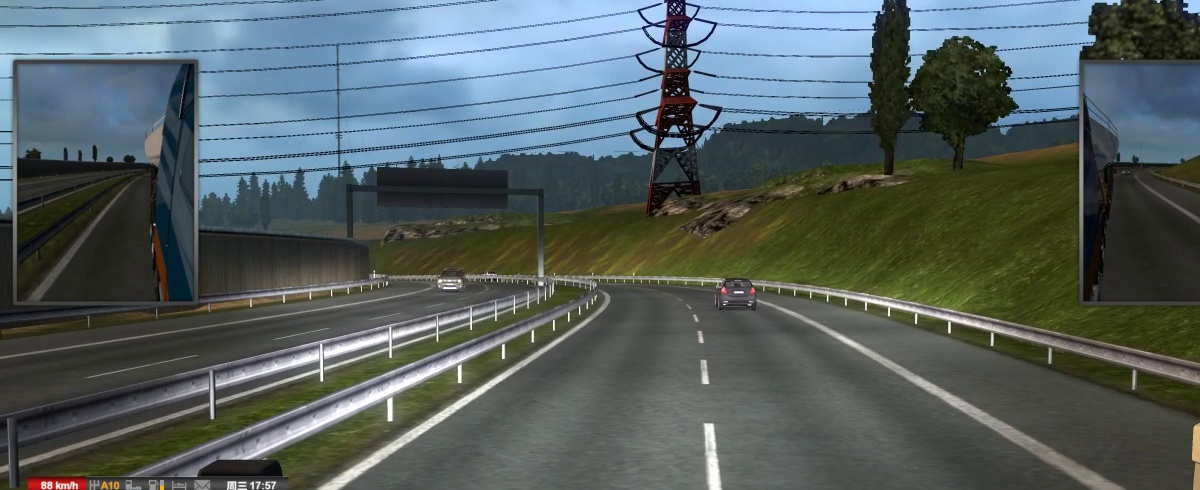
\includegraphics[width=\linewidth]{result/w000059.jpg}
      \caption{Original Image}\label{fig:Original_Image}
    \endminipage\hfill
    \minipage{0.32\textwidth}
      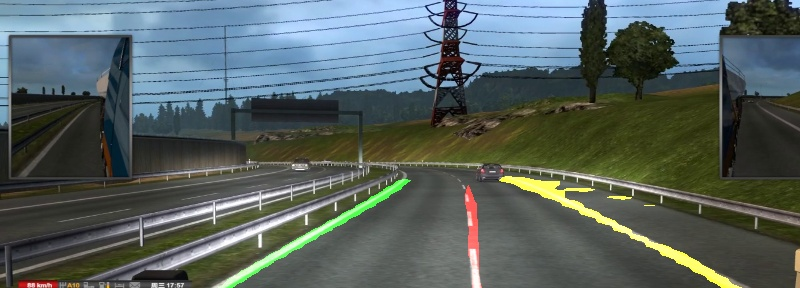
\includegraphics[width=\linewidth]{result/w000059-lane.jpg}
      \caption{Lane Detection}\label{fig:Lane_Line_Result}
    \endminipage\hfill
    \minipage{0.32\textwidth}%
      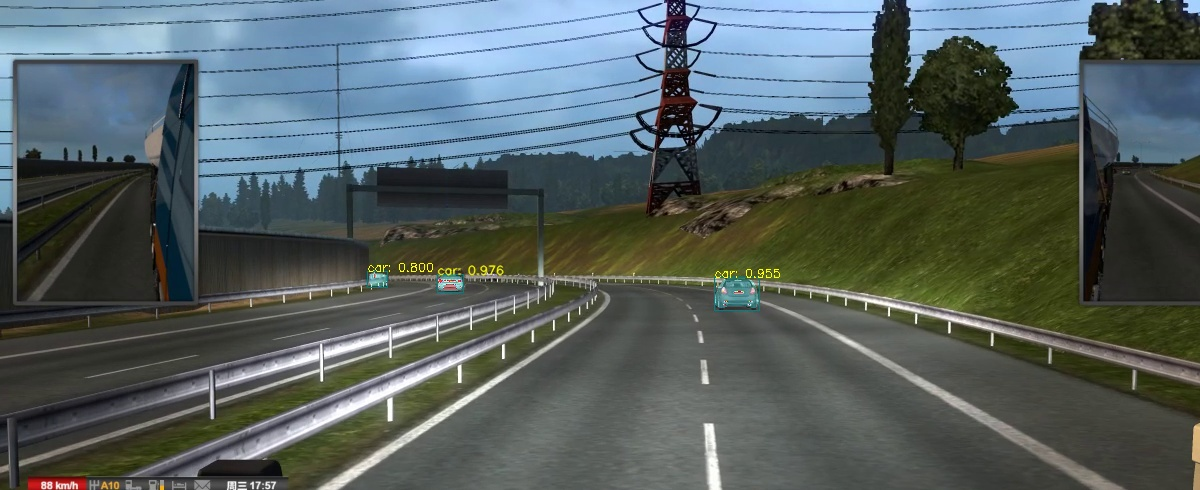
\includegraphics[width=\linewidth]{result/w000059-obj.jpg}
      \caption{Object Detection}\label{fig:Object_result}
    \endminipage
\end{figure}
\begin{figure}[!htb]
	\minipage{0.32\textwidth}
	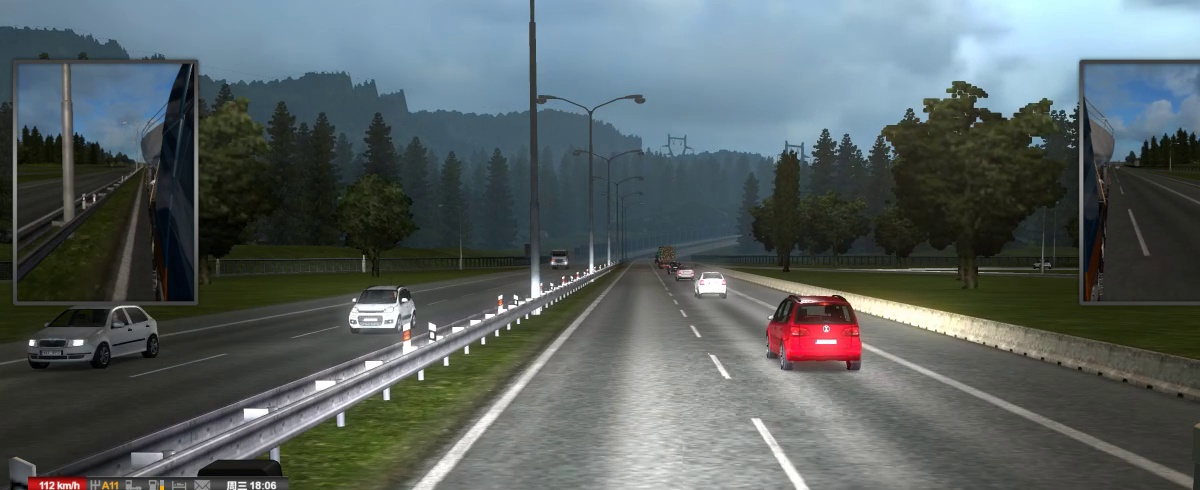
\includegraphics[width=\linewidth]{result/w000066.jpg}
	\caption{Original Image}\label{fig:Original_Image}
	\endminipage\hfill
	\minipage{0.32\textwidth}
	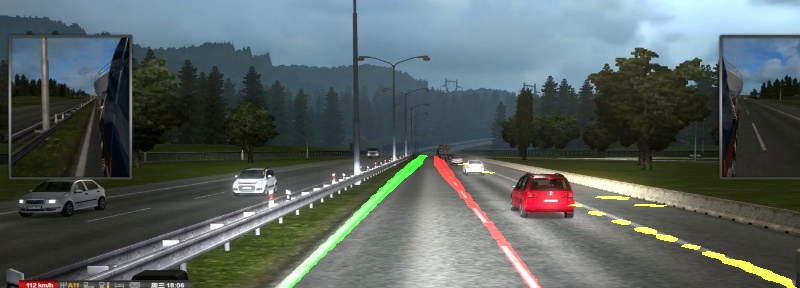
\includegraphics[width=\linewidth]{result/w000066-lane.jpg}
	\caption{Lane Detection}\label{fig:Lane_Line_Result}
	\endminipage\hfill
	\minipage{0.32\textwidth}%
	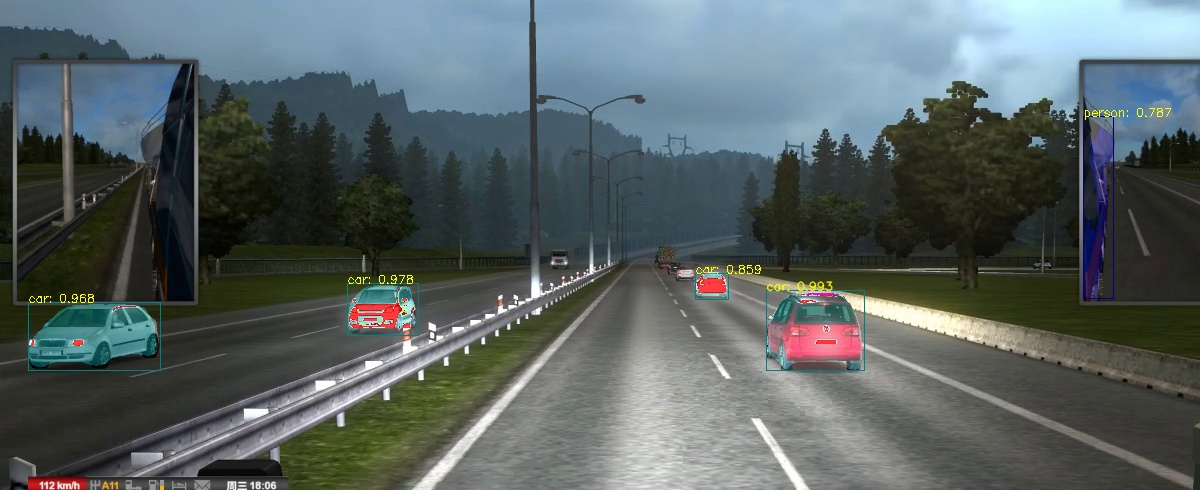
\includegraphics[width=\linewidth]{result/w000066-obj.jpg}
	\caption{Object Detection}\label{fig:Object_result}
	\endminipage
\end{figure}
\begin{figure}[!htb]
	\minipage{0.32\textwidth}
	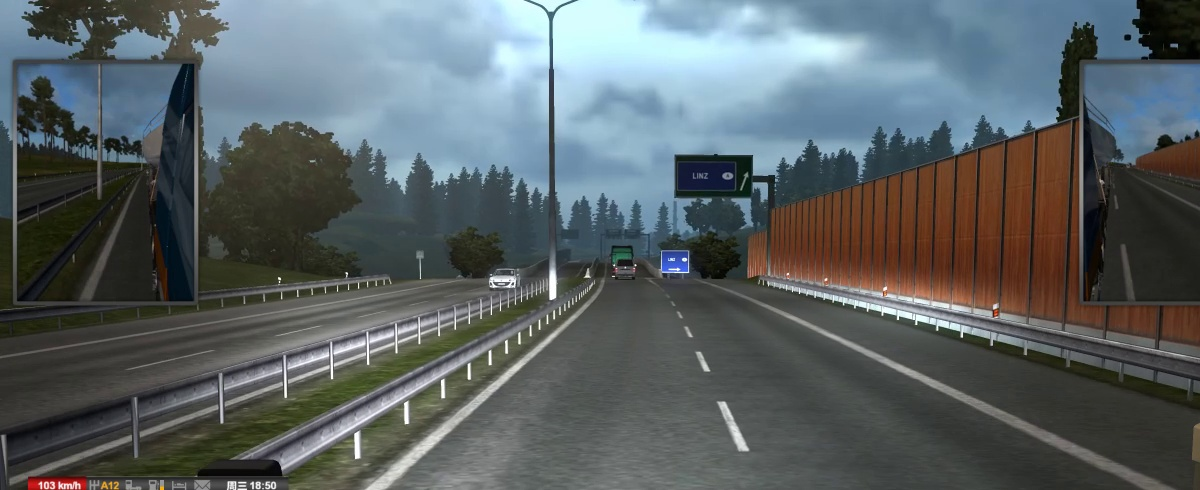
\includegraphics[width=\linewidth]{result/w000092.jpg}
	\caption{Original Image}\label{fig:Original_Image}
	\endminipage\hfill
	\minipage{0.32\textwidth}
	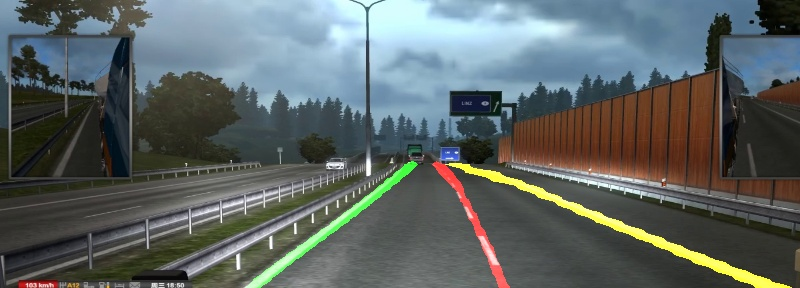
\includegraphics[width=\linewidth]{result/w000092-lane.jpg}
	\caption{Lane Detection}\label{fig:Lane_Line_Result}
	\endminipage\hfill
	\minipage{0.32\textwidth}%
	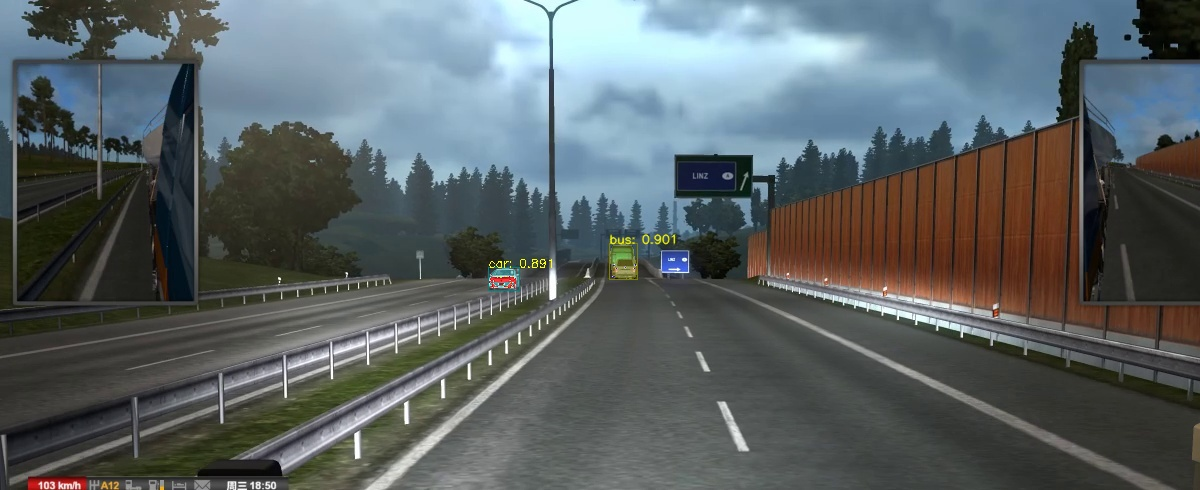
\includegraphics[width=\linewidth]{result/w000092-obj.jpg}
	\caption{Object Detection}\label{fig:Object_result}
	\endminipage
\end{figure}
\begin{figure}[!htb]
	\minipage{0.32\textwidth}
	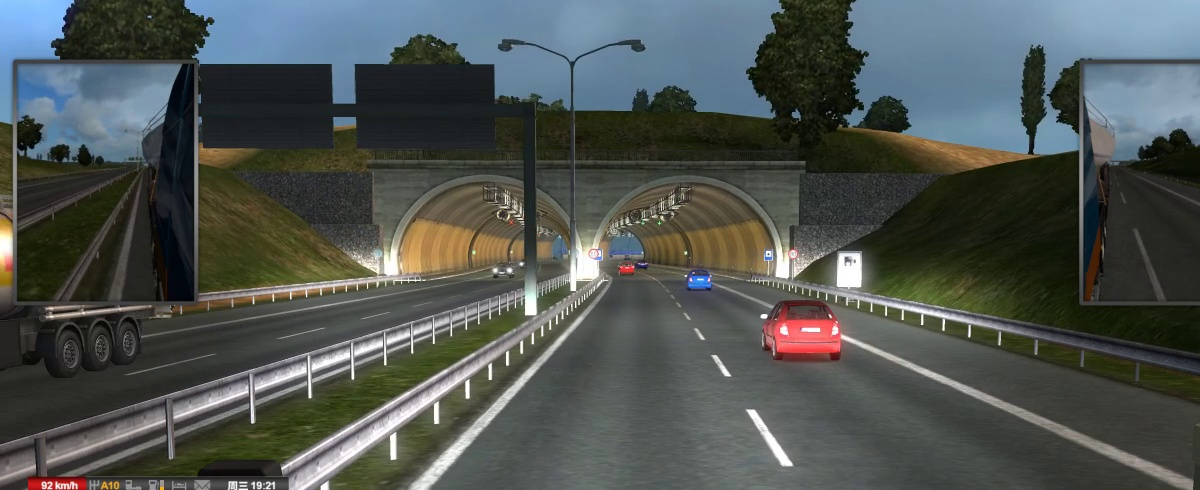
\includegraphics[width=\linewidth]{result/w000106.jpg}
	\caption{Original Image}\label{fig:Original_Image}
	\endminipage\hfill
	\minipage{0.32\textwidth}
	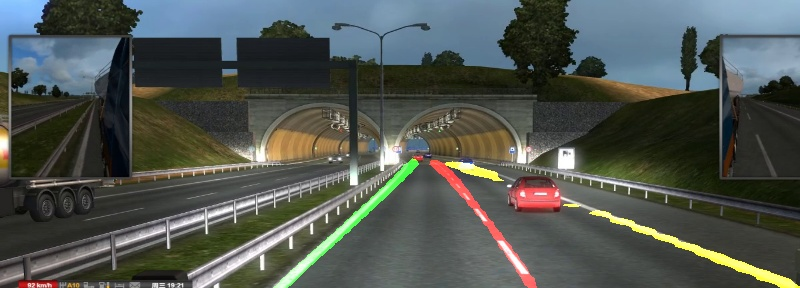
\includegraphics[width=\linewidth]{result/w000106-lane.jpg}
	\caption{Lane Detection}\label{fig:Lane_Line_Result}
	\endminipage\hfill
	\minipage{0.32\textwidth}%
	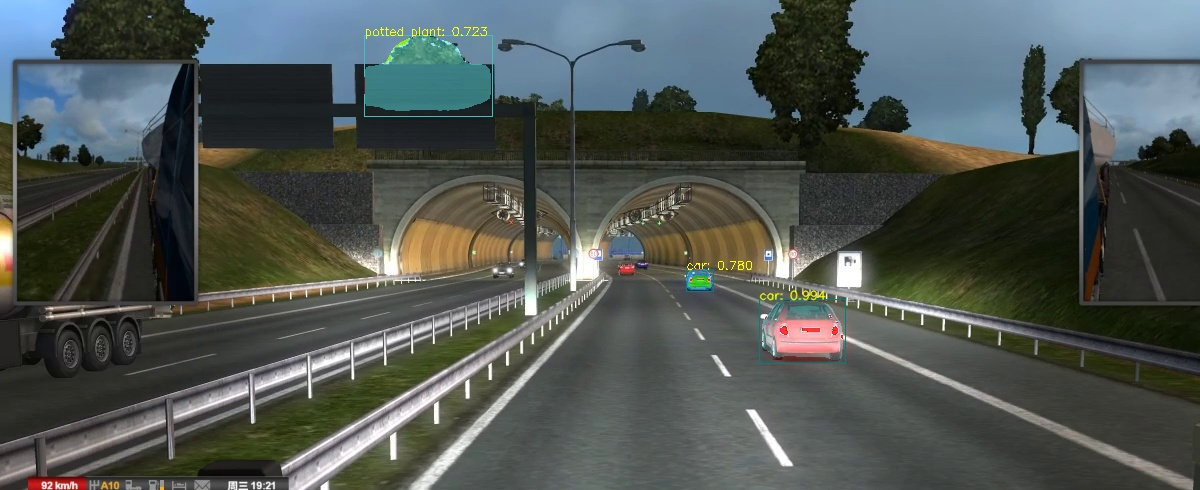
\includegraphics[width=\linewidth]{result/w000106-obj.jpg}
	\caption{Object Detection}\label{fig:Object_result}
	\endminipage
\end{figure}
\begin{figure}[!htb]
	\minipage{0.32\textwidth}
	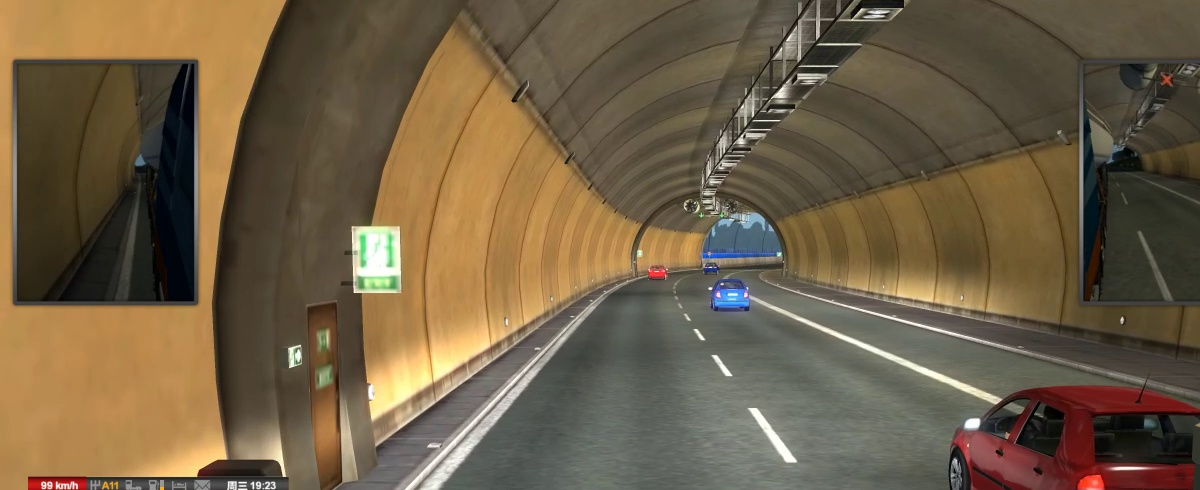
\includegraphics[width=\linewidth]{result/w000107.jpg}
	\caption{Original Image}\label{fig:Original_Image}
	\endminipage\hfill
	\minipage{0.32\textwidth}
	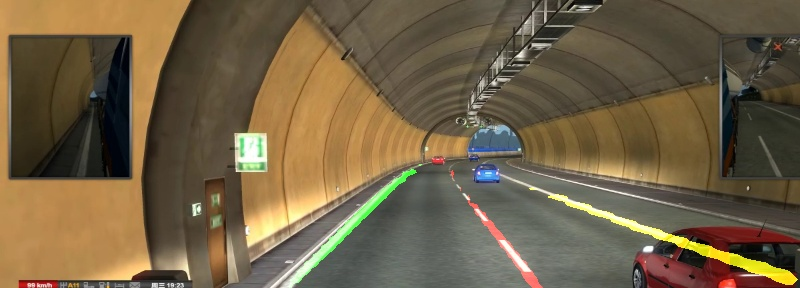
\includegraphics[width=\linewidth]{result/w000107-lane.jpg}
	\caption{Lane Detection}\label{fig:Lane_Line_Result}
	\endminipage\hfill
	\minipage{0.32\textwidth}%
	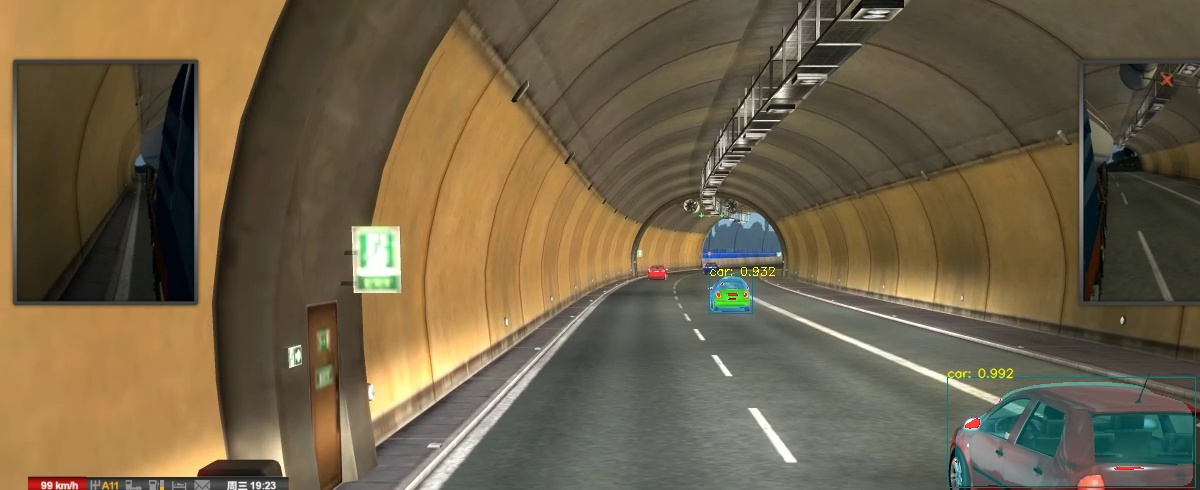
\includegraphics[width=\linewidth]{result/w000107-obj.jpg}
	\caption{Object Detection}\label{fig:Object_result}
	\endminipage
\end{figure}
\begin{figure}[!htb]
	\minipage{0.32\textwidth}
	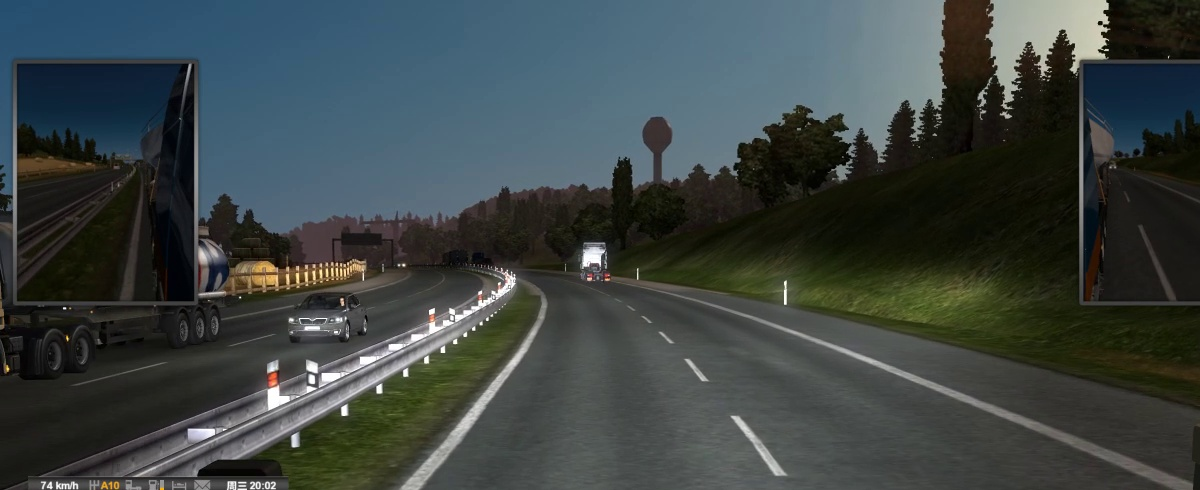
\includegraphics[width=\linewidth]{result/w000128.jpg}
	\caption{Original Image}\label{fig:Original_Image}
	\endminipage\hfill
	\minipage{0.32\textwidth}
	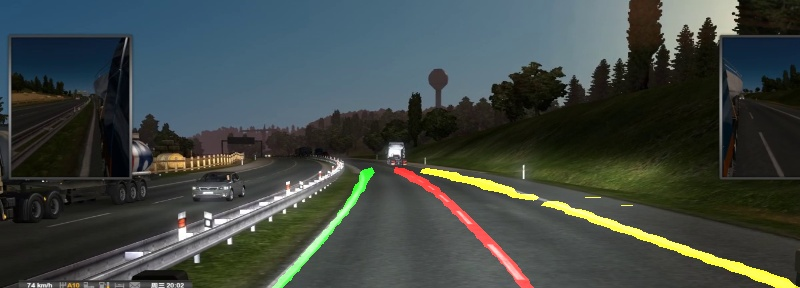
\includegraphics[width=\linewidth]{result/w000128-lane.jpg}
	\caption{Lane Detection}\label{fig:Lane_Line_Result}
	\endminipage\hfill
	\minipage{0.32\textwidth}%
	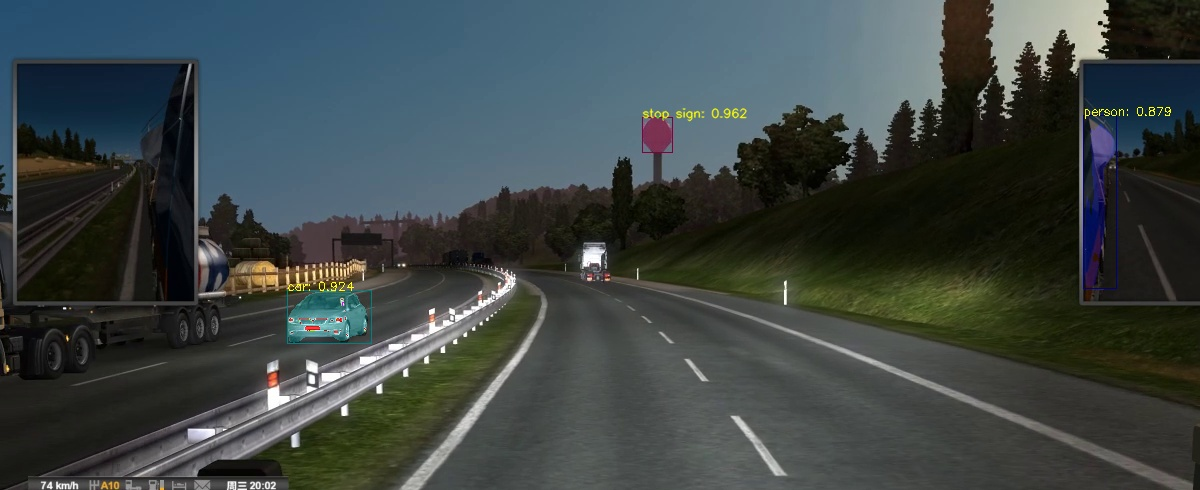
\includegraphics[width=\linewidth]{result/w000128-obj.jpg}
	\caption{Object Detection}\label{fig:Object_result}
	\endminipage
\end{figure}
\begin{figure}[!htb]
	\minipage{0.32\textwidth}
	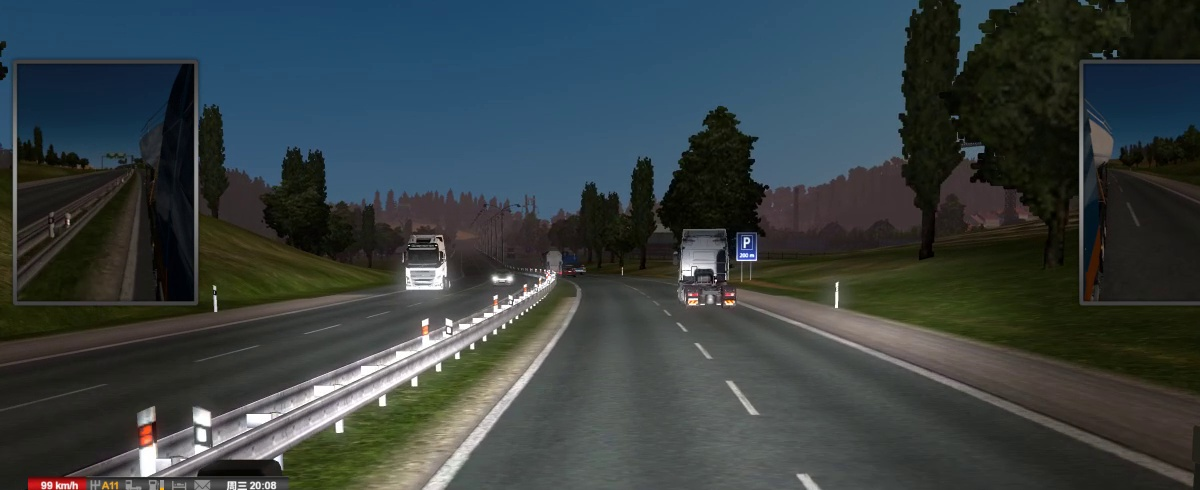
\includegraphics[width=\linewidth]{result/w000131.jpg}
	\caption{Original Image}\label{fig:Original_Image}
	\endminipage\hfill
	\minipage{0.32\textwidth}
	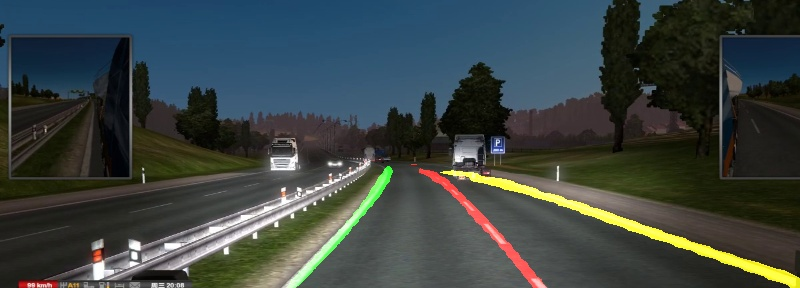
\includegraphics[width=\linewidth]{result/w000131-lane.jpg}
	\caption{Lane Detection}\label{fig:Lane_Line_Result}
	\endminipage\hfill
	\minipage{0.32\textwidth}%
	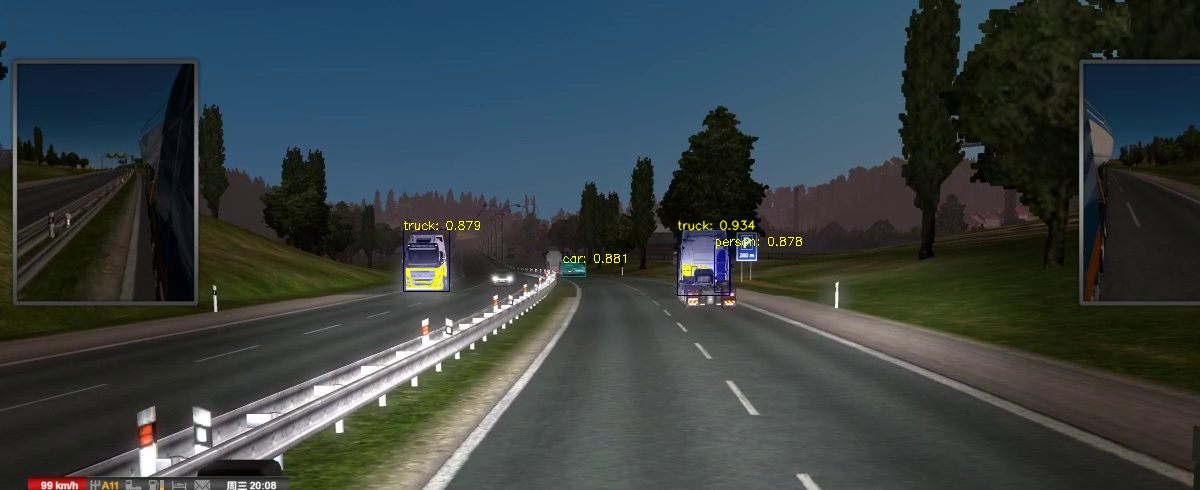
\includegraphics[width=\linewidth]{result/w000131-obj.jpg}
	\caption{Object Detection}\label{fig:Object_result}
	\endminipage
\end{figure}
\begin{figure}[!htb]
	\minipage{0.32\textwidth}
	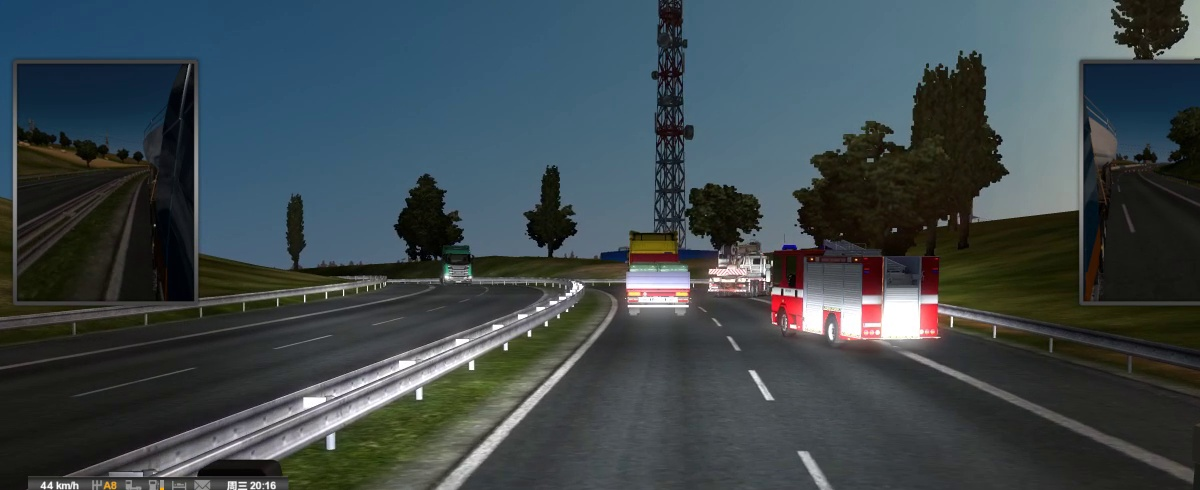
\includegraphics[width=\linewidth]{result/w000139.jpg}
	\caption{Original Image}\label{fig:Original_Image}
	\endminipage\hfill
	\minipage{0.32\textwidth}
	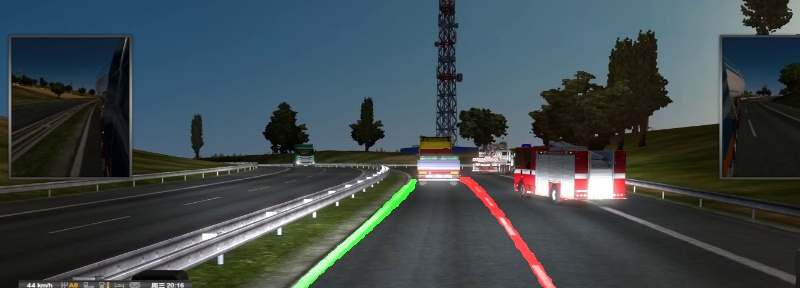
\includegraphics[width=\linewidth]{result/w000139-lane.jpg}
	\caption{Lane Detection}\label{fig:Lane_Line_Result}
	\endminipage\hfill
	\minipage{0.32\textwidth}%
	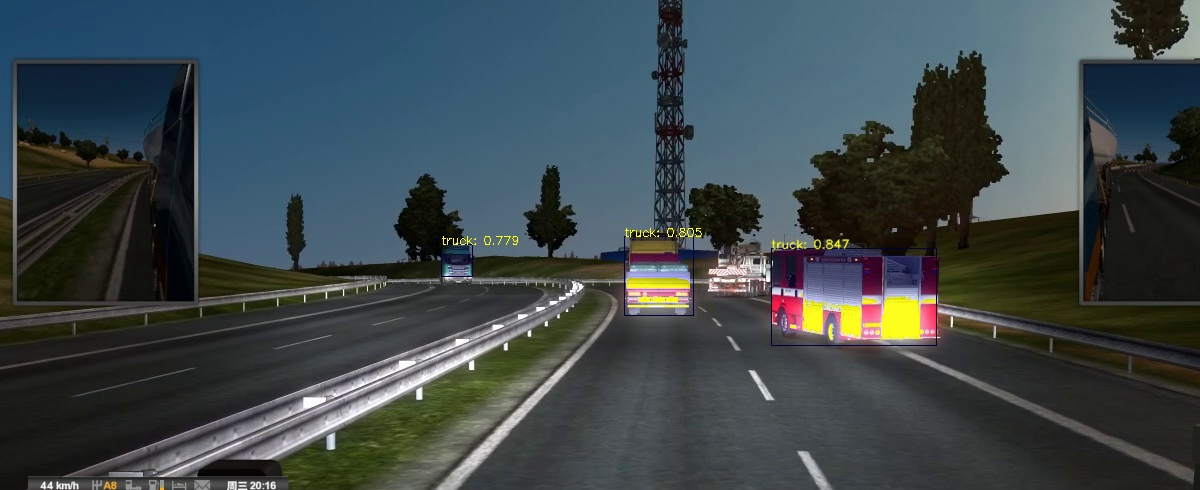
\includegraphics[width=\linewidth]{result/w000139-obj.jpg}
	\caption{Object Detection}\label{fig:Object_result}
	\endminipage
\end{figure}
\clearpage


\bibliographystyle{splncs}
\bibliography{bib}
\end{document}
